\documentclass[12pt,a4paper]{article}

% Компиляция из папки проекта: pdflatex main.tex
\usepackage[T2A]{fontenc}
\usepackage[utf8]{inputenc}
\usepackage[russian]{babel}
\usepackage{amsmath,amssymb}
\usepackage{graphicx}
\usepackage{float}
\usepackage{booktabs}
\usepackage{array}
\usepackage{geometry}
\usepackage{indentfirst}
\usepackage{caption}
\usepackage{url}
\usepackage{tikz}

\geometry{left=2.5cm,right=2.5cm,top=2.5cm,bottom=2.5cm}
\setlength{\parindent}{1.25cm}
\setlength{\parskip}{0pt}
\renewcommand{\arraystretch}{1.2}
\captionsetup{font=small,labelfont=normalfont,labelsep=colon}
\addto\captionsrussian{\renewcommand{\figurename}{Рис.}}

% Изображения для разделов 1--2 лежат в images/ рядом с main.tex.
% Графики раздела 5: images/B_of_H_1.png, B_of_H_2.png, B_of_H_3.png.

\begin{document}

% ------------------------------------------------------------
% ТИТУЛЬНЫЙ ЛИСТ — воспроизводит композицию образца main(2).pdf.
% Абсолютные координаты — в pt от верхнего левого угла страницы A4.
% Меняйте только название, номер работы и данные студента.
% ------------------------------------------------------------
\begin{titlepage}
  \thispagestyle{empty}
  \begin{tikzpicture}[remember picture,overlay]
    % Для образца центр набора смещён на 21 pt вправо от центра A4.
    \coordinate (sheetcenter) at ([xshift=21pt]current page.north);

    % Название института.
    \node[anchor=north,inner sep=0pt,font=\Large]
      at ([yshift=-59pt]sheetcenter)
      {Московский Физико-Технический Институт};

    % Номер работы, над названием.
    \node[anchor=north,inner sep=0pt,font=\Large]
      at ([yshift=-194.6pt]sheetcenter)
      {Лабораторная работа №3.4.5};

    % Горизонтальные линии в точности по ширине набора образца.
    \draw[line width=0.4pt]
      ([xshift=85pt,yshift=-236pt]current page.north west) --
      ([xshift=552pt,yshift=-236pt]current page.north west);

    % Название крупным полужирным шрифтом, в две строки.
    \node[anchor=north,inner sep=0pt,align=center,font=\huge\bfseries]
      at ([yshift=-259pt]sheetcenter)
      {Петля гистерезиса\\[0pt](динамический метод)};

    \draw[line width=0.4pt]
      ([xshift=85pt,yshift=-331pt]current page.north west) --
      ([xshift=552pt,yshift=-331pt]current page.north west);

    % Блок студента в правой нижней части — как в образце.
    \node[anchor=north west,inner sep=0pt,font=\large]
      at ([xshift=357.4pt,yshift=-513.3pt]current page.north west)
      {{\renewcommand{\arraystretch}{0.94}\begin{tabular}{@{}l@{}}
        Выполнил:\\
        Студент 2 курса ФАКТ\\
        Группа Б03-502\\
        Подмосковнов Лев
      \end{tabular}}};

    % Город и год по центру области набора.
    \node[anchor=north,inner sep=0pt,align=center,font=\large]
      at ([yshift=-761.5pt]sheetcenter)
      {Долгопрудный\\[-1pt]2026};
  \end{tikzpicture}
\end{titlepage}

% Страницы основного текста начинаются с 1, как в образце.
\setcounter{page}{1}

\section*{Цель работы}
Изучение петель гистерезиса различных ферромагнитных материалов
в переменных магнитных полях.

\section*{Используемые приборы и материалы}
В работе используются:
\begin{itemize}
  \item автотрансформатор и понижающий трансформатор;
  \item тороидальные образцы с двумя обмотками;
  \item интегрирующая $RC$-цепочка;
  \item амперметр и вольтметр;
  \item электронный осциллограф;
  \item делитель напряжения и соединительные провода.
\end{itemize}

% ------------------------------------------------------------
% 1. ТЕОРИЯ
% ------------------------------------------------------------
\section{Теоретическое введение}

\subsection{Ферромагнитный гистерезис}
Магнитная индукция $B$ в ферромагнетике зависит не только от
напряжённости магнитного поля $H$, но и от предыстории намагничивания
образца. При циклическом изменении поля возникает петля гистерезиса.

Индукция насыщения $B_s$ характеризует магнитную индукцию при достижении
насыщения намагниченности образца. Остаточная индукция $B_r$ ---
индукция при $H=0$ после намагничивания образца. Коэрцитивное поле
$H_c$ --- модуль напряжённости обратного поля, при котором $B=0$.
Площадь петли гистерезиса соответствует энергии, рассеиваемой за цикл
перемагничивания в единице объёма материала.
\begin{figure}[H]
    \centering
    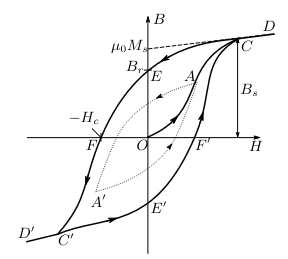
\includegraphics[width=0.5\textwidth]{images/hysteresis_loop.png}
    \caption{Характерная петля гистерезиса ферромагнетика}
    \label{fig:hysteresis}
\end{figure}

\subsection{Измерение напряжённости магнитного поля}
В тороидальном образце напряжённость поля связана с током
$I_0$ в намагничивающей обмотке соотношением
\begin{equation}
  H = \frac{N_0 I_0}{l},
  \label{eq:H}
\end{equation}
где $N_0$~--- число витков намагничивающей обмотки,
$l$~--- средняя длина магнитной линии тороида.

\subsection{Измерение индукции и интегрирующая цепочка}
По закону электромагнитной индукции напряжение на измерительной
обмотке пропорционально скорости изменения магнитной индукции:
\begin{equation}
  |\mathcal{E}| = N_{\text{и}} S\left|\frac{dB}{dt}\right|,
  \label{eq:emf}
\end{equation}
где $N_{\text{и}}$~--- число витков измерительной обмотки,
$S$~--- площадь поперечного сечения образца.

При выполнении условия $\omega_0\tau_{\text{и}}\gg 1$ интегрирующая
$RC$-цепочка позволяет определить индукцию по выходному напряжению:
\begin{equation}
  |B|=\frac{\tau_{\text{и}}}{N_{\text{и}}S}|U_C|,
  \qquad \tau_{\text{и}}=R_{\text{и}}C_{\text{и}}.
  \label{eq:B}
\end{equation}

\subsection{Экспериментальная установка}
Напряжение $U_R$ с резистора $R_0$, включённого последовательно
с намагничивающей обмоткой, подаётся на канал $X$ осциллографа.
Напряжение $U_C$ с интегрирующей цепочки подаётся на канал $Y$.
Поэтому изображение на экране в режиме $X$--$Y$ воспроизводит петлю
гистерезиса в координатах $H$--$B$.

\begin{figure}[H]
    \centering
    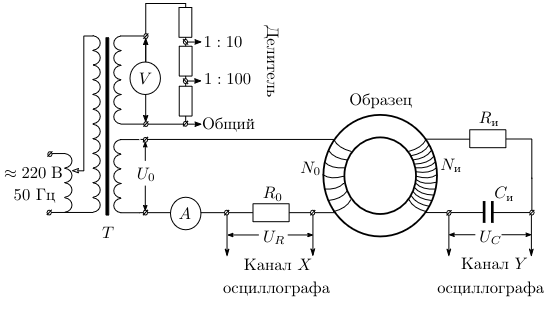
\includegraphics[width=0.85\textwidth]{images/setup.png}
    \caption{Схема установки для исследования намагничивания образцов}
    \label{fig:setup}
\end{figure}

% ------------------------------------------------------------
% 2. ПЕТЛИ ГИСТЕРЕЗИСА
% ------------------------------------------------------------
\section{Измерение петель гистерезиса}

\subsection{Параметры образцов}
% Параметры образцов из экспериментальной тетради.
\begin{table}[H]
  \centering
  \caption{Параметры исследуемых тороидальных образцов}
  \label{tab:samples}
  \begin{tabular}{l c c c c}
    \toprule
    Материал & $N_0$ & $N_{\text{и}}$ & $l$, см & $S$, см$^2$ \\
    \midrule
    Кремнистое железо Fe--Si & 35 & 350 & 10 & 1,2 \\
    Пермаллой Fe--Ni НП50 & 35 & 220 & 24 & 3,8 \\
    Феррит 1000НН & 45 & 400 & 25 & 3,0 \\
    \bottomrule
  \end{tabular}
\end{table}

Далее в таблицах приняты сокращения: Fe--Si --- кремнистое железо,
НП50 --- пермаллой Fe--Ni НП50, 1000НН --- феррит 1000НН.

\subsection{Предельные петли гистерезиса}
% Для каждого образца: фото петли, K_x, K_y, действующее значение I,
% 2X_s, 2Y_s, 2X_c, 2Y_r. Если образцов больше/меньше, изменить таблицу.

В таблице приведены действующие значения тока $I$,
установленные на осциллографе масштабы $K_x$, $K_y$
и размеры петель в делениях экрана. Координаты
$2X_s$, $2Y_s$, $2X_c$ и $2Y_r$ измерялись по полным
ширинам и высотам соответствующих участков.

\begin{table}[H]
    \centering
    \caption{Результаты измерения предельных петель гистерезиса}
    \label{tab:hysteresis}
    \scriptsize
    \setlength{\tabcolsep}{3.1pt}
    \begin{tabular}{|c|c|c|c|c|c|c|c|}
        \hline
        Материал &
        $I$, А &
        $K_x$, мВ/дел. &
        $K_y$, мВ/дел. &
        $2X_s$, дел. &
        $2Y_s$, дел. &
        $2X_c$, дел. &
        $2Y_r$, дел. \\
        \hline
        Fe--Si & 0,393 & 50 & 50 & 4,6 & 4,6 & 1,4 & 2,8 \\
        \hline
        НП50 & 0,153 & 10 & 50 & 8,0 & 7,0 & 6,6 & 6,8 \\
        \hline
        1000НН & 0,036 & 10 & 10 & 3,6 & 5,8 & 2,0 & 3,8 \\
        \hline
    \end{tabular}
\end{table}


\begin{figure}[H]
    \centering
    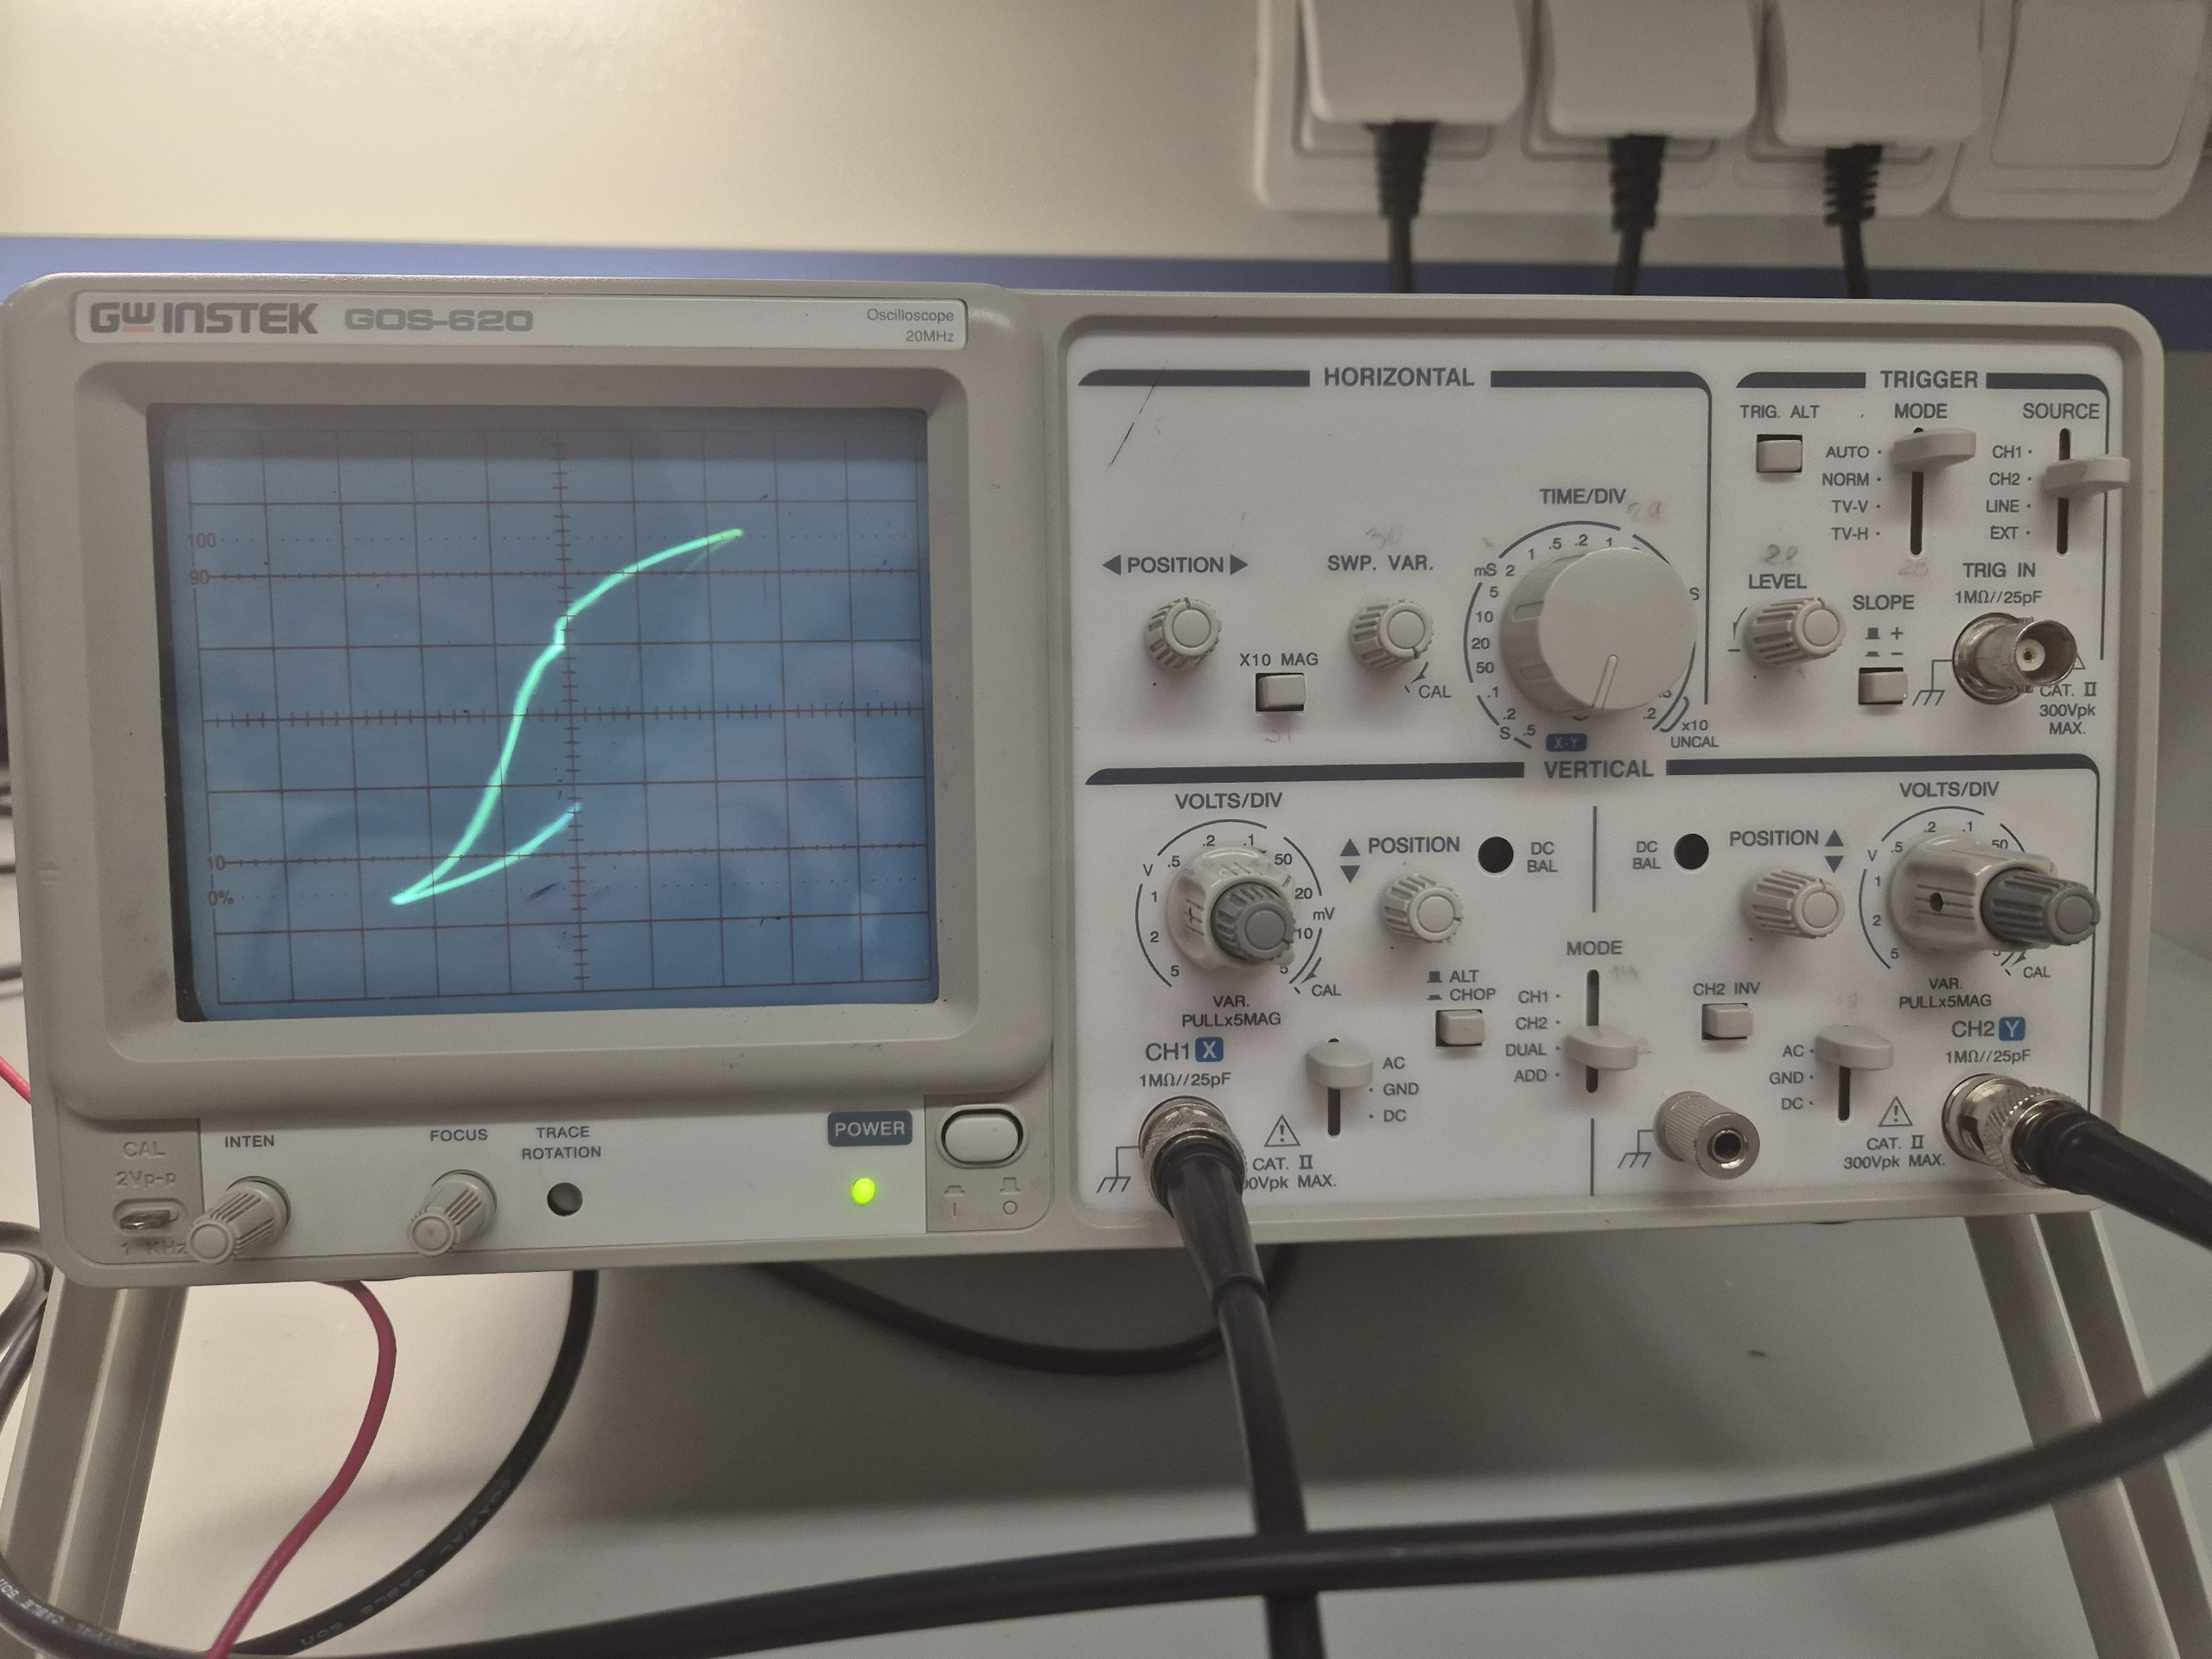
\includegraphics[width=0.78\textwidth]{images/loop_sample_1.png}
    \caption{Наблюдаемая петля гистерезиса кремнистого железа Fe--Si}
    \label{fig:loop1}
\end{figure}



\subsection{Начальные кривые намагничивания}

Для получения начальных кривых намагничивания
постепенно уменьшалась амплитуда тока в
намагничивающей обмотке от значения,
соответствующего предельной петле, до нуля.

Для каждого образца фиксировались координаты
крайних точек частных петель гистерезиса. В таблицах 3--5
приведены непосредственно измеренные отклонения $X$ и $Y$;
перевод в $H$ и $B$ выполняется после калибровки осциллографа
и определения постоянной времени интегрирующей цепочки.

\begin{table}[H]
    \centering
    \caption{Начальная кривая намагничивания
    кремнистого железа Fe-Si}
    \label{tab:initial_1}
    \begin{tabular}{|c|c|c|}
        \hline
        № & $X$, дел. & $Y$, дел. \\
        \hline
        1 & 2,5 & 2,5 \\
        2 & 2,1 & 2,4 \\
        3 & 1,6 & 2,0 \\
        4 & 1,4 & 1,8 \\
        5 & 1,2 & 1,6 \\
        6 & 1,0 & 1,4 \\
        7 & 0,8 & 1,2 \\
        8 & 0,7 & 1,0 \\
        \hline
    \end{tabular}
\end{table}

\begin{table}[H]
    \centering
    \caption{Начальная кривая намагничивания
    пермаллоя Fe-Ni НП50}
    \label{tab:initial_2}
    \begin{tabular}{|c|c|c|}
        \hline
        № & $X$, дел. & $Y$, дел. \\
        \hline
        1 & 3,9 & 3,5 \\
        2 & 3,2 & 3,0 \\
        3 & 3,0 & 2,7 \\
        4 & 2,8 & 2,0 \\
        5 & 2,6 & 1,4 \\
        6 & 2,4 & 1,2 \\
        7 & 2,4 & 1,0 \\
        8 & 2,3 & 0,6 \\
        \hline
    \end{tabular}
\end{table}

\begin{table}[H]
    \centering
    \caption{Начальная кривая намагничивания
    феррита 1000НН}
    \label{tab:initial_3}
    \begin{tabular}{|c|c|c|}
        \hline
        № & $X$, дел. & $Y$, дел. \\
        \hline
        1 & 2,1 & 3,1 \\
        2 & 1,5 & 2,6 \\
        3 & 1,2 & 2,4 \\
        4 & 1,1 & 2,2 \\
        5 & 1,0 & 1,6 \\
        6 & 0,9 & 1,3 \\
        7 & 0,8 & 1,0 \\
        8 & 0,7 & 0,8 \\
        \hline
    \end{tabular}
\end{table}


% ------------------------------------------------------------
% 3. КАЛИБРОВКА И RC-ЦЕПОЧКА
% ------------------------------------------------------------


\section{Калибровка осциллографа}

\subsection{Калибровка горизонтальной оси}

Для определения масштаба по оси $X$ намагничивающая обмотка
закорачивалась. При этом ток имел синусоидальную форму.
Измерялись действующее значение тока $I_{\text{эфф}}$ и полная
ширина горизонтальной развёртки $2X_{\text{кал}}$.
Сопротивление измерительного резистора:
\[
R_0=0{,}2\ \text{Ом}.
\]

Амплитуда напряжения на резисторе $R_0$ равна
$U_{R,\max}=\sqrt{2}R_0 I_{\text{эфф}}$. Поэтому
коэффициент перевода делений в напряжение определяется формулой
\begin{equation}
 k_X=\frac{2\sqrt{2}\,R_0I_{\text{эфф}}}{2X_{\text{кал}}}.
 \label{eq:kx_cal}
\end{equation}
Здесь $k_X$ --- измеренный коэффициент, а $K_x$ ---
номинальное положение переключателя осциллографа.

\begin{table}[H]
 \centering
 \caption{Калибровка горизонтальной оси осциллографа}
 \label{tab:cal_x}
 \small
 \setlength{\tabcolsep}{5pt}
 \begin{tabular}{|c|c|c|c|c|}
 \hline
 Материал & $K_x$, мВ/дел. & $I_{\text{эфф}}$, А &
 $2X_{\text{кал}}$, дел. & $k_X$, мВ/дел. \\
 \hline
 Fe--Si & 50 & 0,883 & 10,0 & 50 \\
 \hline
 НП50 & 10 & 0,115 & 9,2 & 7,1 \\
 \hline
 1000НН & 10 & 0,120 & 9,2 & 7,4 \\
 \hline
 \end{tabular}
\end{table}

Например, для кремнистого железа после перевода результата в мВ/дел.:
\[
 k_X=\frac{2\sqrt{2}\cdot 0{,}2\cdot 0{,}883}{10{,}0}
 \cdot 10^3=50\ \text{мВ/дел.}
\]

\subsection{Проверка калибровки вертикальной оси}

Для проверки вертикальной оси измерялись действующее
напряжение $U_{\text{эфф}}$ и полная высота развёртки
$2Y_{\text{кал}}$. Для синусоидального сигнала:
\begin{equation}
 k_Y=\frac{2\sqrt{2}\,U_{\text{эфф}}}{2Y_{\text{кал}}}.
 \label{eq:ky_cal}
\end{equation}

\begin{table}[H]
 \centering
 \caption{Калибровка вертикальной оси осциллографа}
 \label{tab:cal_y}
 \small
 \setlength{\tabcolsep}{5pt}
 \begin{tabular}{|c|c|c|c|c|}
 \hline
 $K_y$, мВ/дел. & $2Y_{\text{кал}}$, дел. &
 $U_{\text{эфф}}$, мВ & $k_Y$, мВ/дел. &
 $\delta_Y$, \% \\
 \hline
 50 & 7,9 & 125 & 45 & 11 \\
 \hline
 10 & 7,8 & 28,2 & 10 & 2 \\
 \hline
 \end{tabular}
\end{table}

Относительное отклонение измеренного масштаба
от установленного определялось по формуле:
\begin{equation}
 \delta_Y=\frac{|k_Y-K_y|}{K_y}\cdot100\%.
 \label{eq:dy_cal}
\end{equation}

\section{Определение параметров RC-цепочки}

Постоянную времени $RC$-цепочки определяли по отношению
амплитуд входного и выходного синусоидальных сигналов.
При отсутствии нагрузки на выходе для идеальной цепочки
получаем соотношение
\begin{equation}
 \frac{U_{\text{вых}}}{U_{\text{вх}}}
 =\frac{1}{\sqrt{1+(\omega_0\tau_{\text{и}})^2}},
 \qquad \tau_{\text{и}}=R_{\text{и}}C_{\text{и}}.
 \label{eq:rc_ratio}
\end{equation}
Отсюда постоянная времени вычисляется без дополнительного
приближения:
\begin{equation}
 \tau_{\text{эксп}}=\frac{1}{\omega_0}
 \sqrt{\left(\frac{U_{\text{вх}}}{U_{\text{вых}}}\right)^2-1}.
 \label{eq:tau_exact}
\end{equation}

Измеренные и заданные величины:
\[
 U_{\text{вх}}=16\ \text{В},\qquad
 U_{\text{вых}}=124\ \text{мВ}=0{,}124\ \text{В},
\]
\[
 \nu_0=50\ \text{Гц},\qquad
 \omega_0=2\pi\nu_0=100\pi\ \text{рад/с}.
\]
Подстановка измеренных значений даёт:
\[
 \tau_{\text{эксп}}
 =\frac{1}{100\pi}
 \sqrt{\left(\frac{16}{0{,}124}\right)^2-1}
 =0{,}41\ \text{с}.
\]

Параметры интегрирующей цепочки:
\[
 R_{\text{и}}=20\ \text{кОм},\qquad
 C_{\text{и}}=20\ \text{мкФ}.
\]
Расчётное значение постоянной времени:
\begin{equation}
 \tau_{\text{расч}}=R_{\text{и}}C_{\text{и}}
 =20\cdot10^3\cdot20\cdot10^{-6}
 =0{,}40\ \text{с}.
 \label{eq:tau_rc}
\end{equation}

Относительное расхождение между экспериментальным и
расчётным значениями:
\begin{equation}
 \varepsilon=\frac{|\tau_{\text{эксп}}-\tau_{\text{расч}}|}
 {\tau_{\text{расч}}}\cdot100\%=3\%.
 \label{eq:rc_diff}
\end{equation}

Проверим условие интегрирования сигнала:
\[
\omega_0\tau_{\text{расч}}=40\pi\gg1.
\]
Следовательно, интегрирующая цепочка работает в требуемом режиме.

% ------------------------------------------------------------
% 5. ОБРАБОТКА РЕЗУЛЬТАТОВ (дополнить позднее)
% ------------------------------------------------------------
\section{Обработка результатов}

\subsection{Коэффициенты преобразования координат}

Для построения зависимостей $B(H)$ необходимо перейти от отклонений
луча осциллографа $X$ и $Y$, измеренных в делениях, к напряжённости
магнитного поля $H$ и магнитной индукции $B$.

Напряжение на измерительном резисторе и ток намагничивающей обмотки
определяются через экспериментальный коэффициент калибровки $k_X$:
\[
 U_R=k_X X, \qquad I_0=\frac{U_R}{R_0}.
\]
Для тороидального образца получаем
\begin{equation}
 H=\frac{N_0}{l}\,\frac{k_X}{R_0}X=\alpha_H X,
 \qquad \alpha_H=\frac{N_0 k_X}{lR_0}.
 \label{eq:alphaH}
\end{equation}

Выходное напряжение интегрирующей цепочки связано с отклонением
по вертикальной оси соотношением $U_C=k_Y Y$. Тогда
\begin{equation}
 B=\frac{\tau_{\text{и}}k_Y}{N_{\text{и}}S}Y=\alpha_B Y,
 \qquad \alpha_B=\frac{\tau_{\text{и}}k_Y}{N_{\text{и}}S}.
 \label{eq:alphaB}
\end{equation}
Знаки величин $H$ и $B$ выбираются в соответствии с направлениями
осей на экране осциллографа. Здесь $R_0=0{,}2$~Ом,
$\tau_{\text{и}}=0{,}41$~с; длины $l$ и площади $S$ переведены
в единицы СИ. В формулах коэффициенты $k_X$ и $k_Y$
использованы в В/дел.

Для кремнистого железа Fe--Si расчёт даёт
\[
 \alpha_H=
 \frac{35}{0{,}10\cdot0{,}2}\,
 \frac{2\sqrt{2}\cdot0{,}2\cdot0{,}883}{10{,}0}
 =87\ \frac{\text{А}}{\text{м}\cdot\text{дел.}},
\]
\[
 \alpha_B=
 \frac{0{,}41}{350\cdot1{,}2\cdot10^{-4}}\,
 \frac{2\sqrt{2}\cdot125\cdot10^{-3}}{7{,}9}
 =0{,}44\ \frac{\text{Тл}}{\text{дел.}}.
\]

Аналогично рассчитаны коэффициенты для остальных образцов.
\begin{table}[H]
 \centering
 \caption{Коэффициенты преобразования координат осциллографа}
 \label{tab:coord_conversion}
 \small
 \setlength{\tabcolsep}{5pt}
 \begin{tabular}{|c|c|c|c|c|}
 \hline
 Материал & $k_X$, мВ/дел. & $k_Y$, мВ/дел. &
 $\alpha_H$, А/(м$\cdot$дел.) & $\alpha_B$, Тл/дел. \\
 \hline
 Fe--Si & 50 & 45 & 87 & 0,44 \\
 \hline
 НП50 & 7,1 & 45 & 5,2 & 0,22 \\
 \hline
 1000НН & 7,4 & 10 & 6,6 & 0,035 \\
 \hline
 \end{tabular}
\end{table}

Следовательно, для исследуемых образцов получены соотношения:
\begin{align*}
 \text{Fe--Si:}\quad &H=87X,   & B=0{,}44Y;\\
 \text{НП50:}\quad &H=5{,}2X, & B=0{,}22Y;\\
 \text{1000НН:}\quad &H=6{,}6X, & B=0{,}035Y.
\end{align*}
Здесь $X$ и $Y$ выражены в делениях, $H$ --- в А/м,
$B$ --- в Тл. Погрешности будут оценены в п.~5.5.

\subsection{Индукция насыщения, коэрцитивное поле и остаточная индукция}

По результатам измерения предельных петель гистерезиса
(табл.~\ref{tab:hysteresis}) определялись амплитуда напряжённости
магнитного поля $H_{\max}$, индукция насыщения $B_s$,
коэрцитивное поле $H_c$ и остаточная индукция $B_r$.

Значения $2X_s$ и $2Y_s$ задают полные ширину и высоту
предельной петли, а $2X_c$ и $2Y_r$ --- удвоенные координаты
её пересечений с осями. Поэтому, используя коэффициенты
преобразования из табл.~\ref{tab:coord_conversion}, получаем:
\begin{align}
 H_{\max}&=\alpha_H\frac{2X_s}{2}, &
 B_s&=\alpha_B\frac{2Y_s}{2}, \label{eq:saturation_params}\\
 H_c&=\alpha_H\frac{2X_c}{2}, &
 B_r&=\alpha_B\frac{2Y_r}{2}. \label{eq:remanence_params}
\end{align}

Например, для кремнистого железа Fe--Si расчёт даёт:
\begin{align*}
 H_{\max}&=\alpha_H\cdot\frac{4{,}6}{2}
             =200\ \text{А/м},\\
 B_s&=\alpha_B\cdot\frac{4{,}6}{2}
             =1{,}0\ \text{Тл},\\
 H_c&=\alpha_H\cdot\frac{1{,}4}{2}
             =61\ \text{А/м},\\
 B_r&=\alpha_B\cdot\frac{2{,}8}{2}
             =0{,}61\ \text{Тл}.
\end{align*}

Аналогичные вычисления проведены для остальных образцов.
\begin{table}[H]
  \centering
  \caption{Магнитные характеристики исследуемых материалов}
  \label{tab:results}
  \begin{tabular}{c c c c c}
    \toprule
    Материал & $H_{\max}$, А/м & $B_s$, Тл & $H_c$, А/м & $B_r$, Тл \\
    \midrule
    Fe--Si & 200 & 1,0 & 61 & 0,61 \\
    НП50 & 21 & 0,77 & 17 & 0,75 \\
    1000НН & 12 & 0,10 & 6,6 & 0,066 \\
    \bottomrule
  \end{tabular}
\end{table}

\subsection{Начальные кривые намагничивания}

По измеренным отклонениям $X$ и $Y$ из таблиц~\ref{tab:initial_1}--\ref{tab:initial_3}
рассчитаны напряжённость $H$ и индукция $B$ для всех трёх образцов.
Использовались соотношения из п.~5.1:
\begin{equation}
  H=\alpha_H X, \qquad B=\alpha_B Y.
\end{equation}

Например, для первой точки кремнистого железа Fe--Si ($X=2{,}5$, $Y=2{,}5$):
\begin{align*}
 H_1 &= \frac{35}{0{,}10\cdot0{,}2}
 \frac{2\sqrt{2}\cdot0{,}2\cdot0{,}883}{10{,}0}
 \cdot 2{,}5 = 220\ \text{А/м},\\
 B_1 &= \frac{\tau_{\text{эксп}}}{350\cdot1{,}2\cdot10^{-4}}
 \frac{2\sqrt{2}\cdot125\cdot10^{-3}}{7{,}9}
 \cdot2{,}5 = 1{,}1\ \text{Тл}.
\end{align*}

\begin{table}[H]
  \centering
  \caption{Рассчитанные точки начальной кривой намагничивания кремнистого железа Fe--Si}
  \label{tab:HB_1}
  \begin{tabular}{c c c}
    \toprule
    № точки & $H$, А/м & $B$, Тл \\
    \midrule
    1 & 220 & 1,1 \\
    2 & 180 & 1,1 \\
    3 & 140 & 0,88 \\
    4 & 120 & 0,79 \\
    5 & 100 & 0,70 \\
    6 & 87 & 0,61 \\
    7 & 70 & 0,53 \\
    8 & 61 & 0,44 \\
    \bottomrule
  \end{tabular}
\end{table}
\begin{figure}[H]
  \centering
  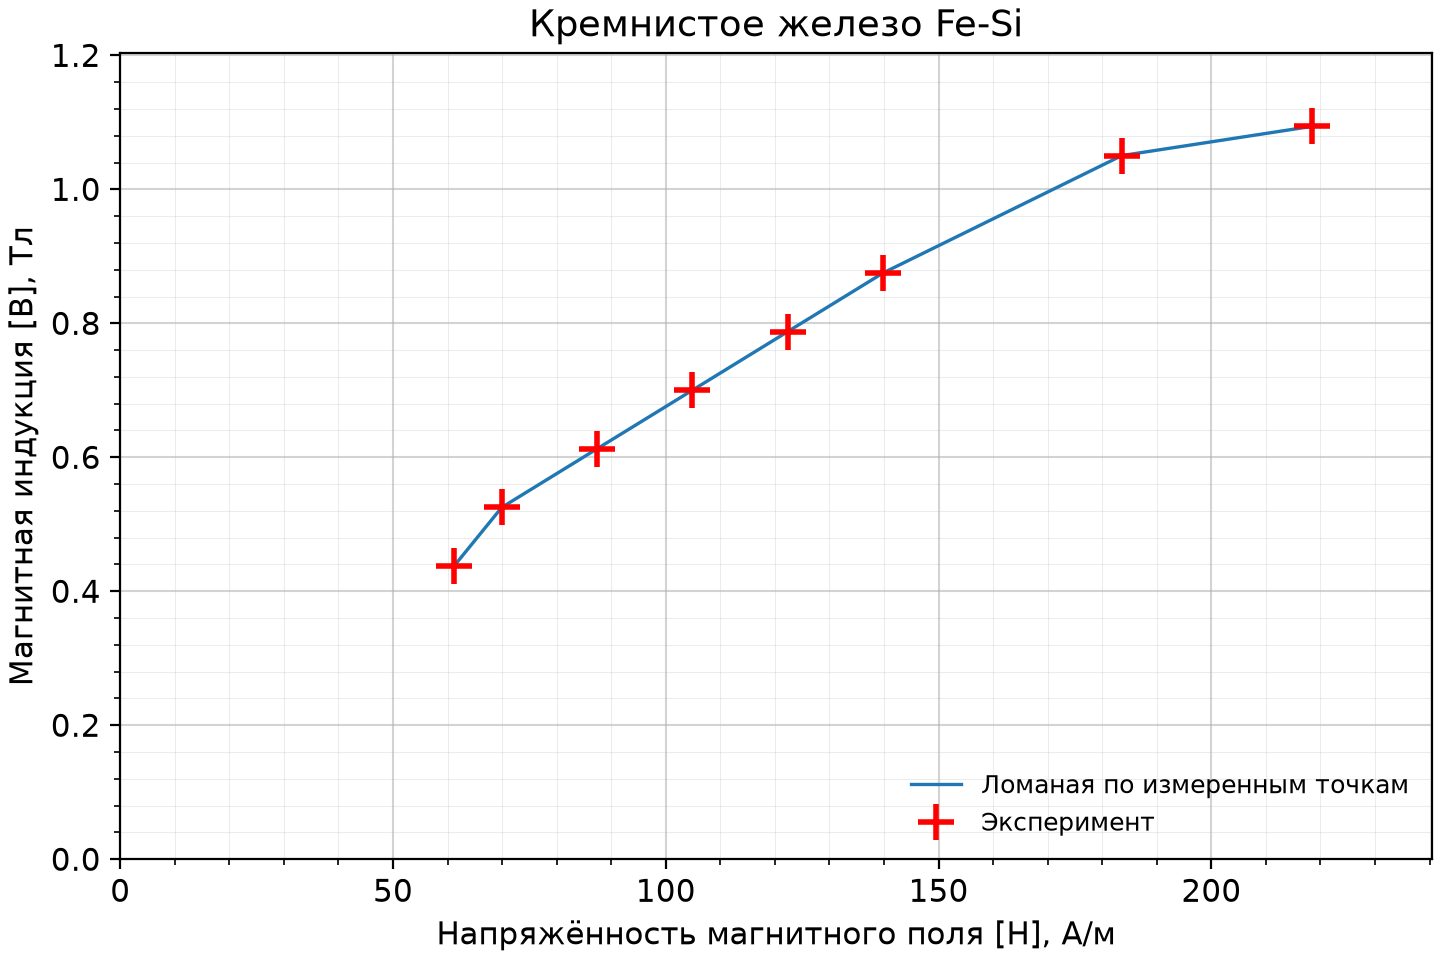
\includegraphics[width=0.85\textwidth]{images/B_of_H_1.png}
  \caption{Начальная кривая намагничивания (экспериментальные точки и соединяющие отрезки) кремнистого железа Fe--Si $B(H)$}
  \label{fig:BH_1}
\end{figure}

\begin{table}[H]
  \centering
  \caption{Рассчитанные точки начальной кривой намагничивания пермаллоя Fe--Ni НП50}
  \label{tab:HB_2}
  \begin{tabular}{c c c}
    \toprule
    № точки & $H$, А/м & $B$, Тл \\
    \midrule
    1 & 20 & 0,77 \\
    2 & 16 & 0,66 \\
    3 & 15 & 0,59 \\
    4 & 14 & 0,44 \\
    5 & 13 & 0,31 \\
    6 & 12 & 0,26 \\
    7 & 12 & 0,22 \\
    8 & 12 & 0,13 \\
    \bottomrule
  \end{tabular}
\end{table}
\begin{figure}[H]
  \centering
  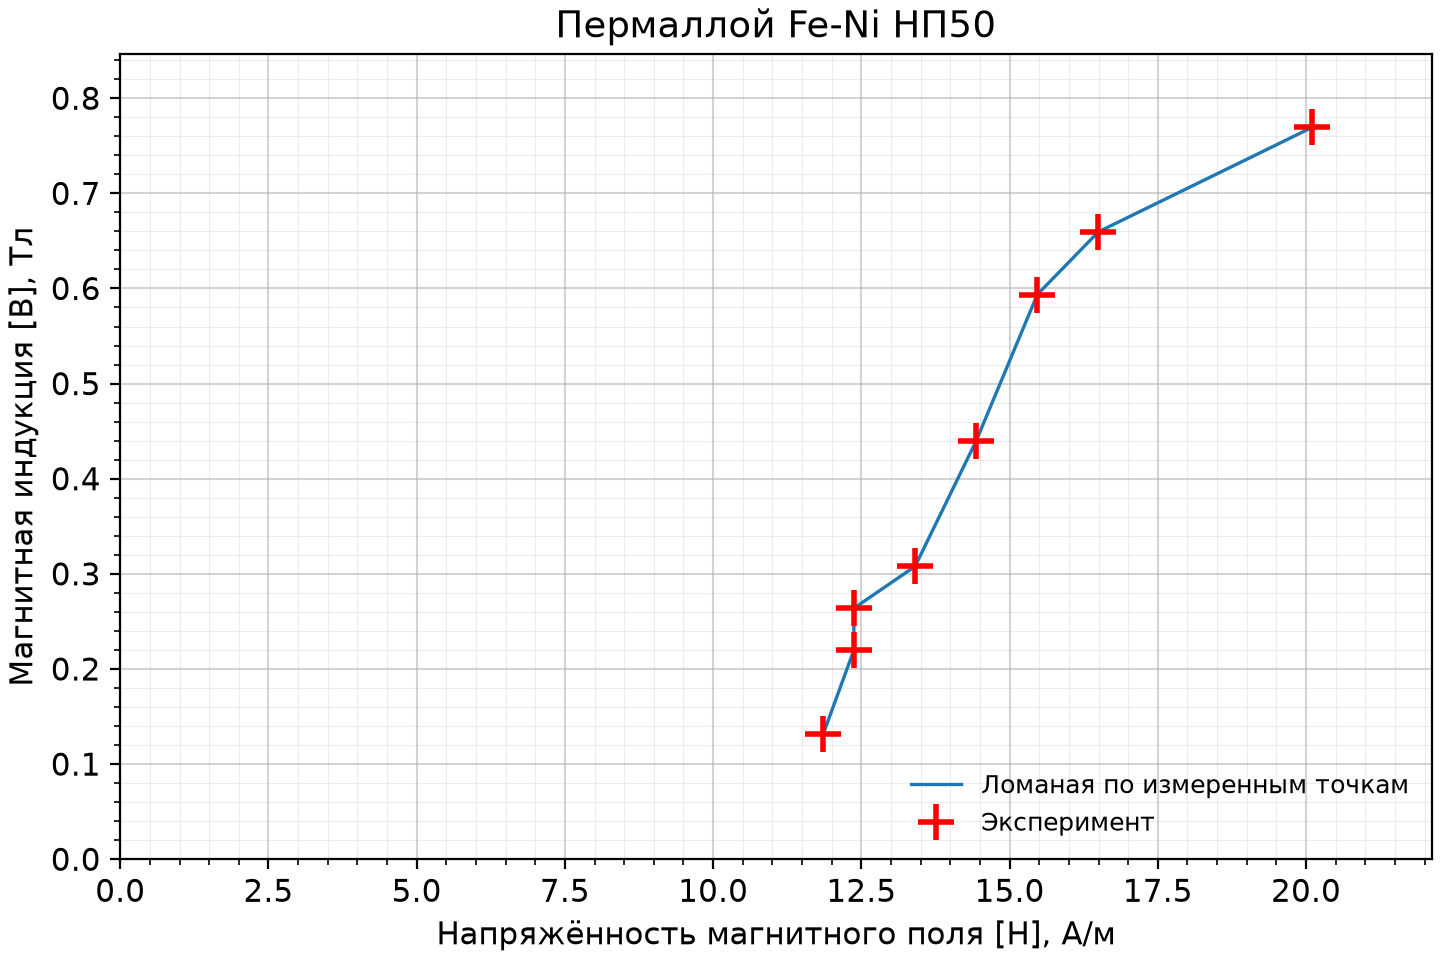
\includegraphics[width=0.85\textwidth]{images/B_of_H_2.png}
  \caption{Начальная кривая намагничивания (экспериментальные точки и соединяющие отрезки) пермаллоя Fe--Ni НП50 $B(H)$}
  \label{fig:BH_2}
\end{figure}

\begin{table}[H]
  \centering
  \caption{Рассчитанные точки начальной кривой намагничивания феррита 1000НН}
  \label{tab:HB_3}
  \begin{tabular}{c c c}
    \toprule
    № точки & $H$, А/м & $B$, Тл \\
    \midrule
    1 & 14 & 0,11 \\
    2 & 10 & 0,091 \\
    3 & 8,0 & 0,084 \\
    4 & 7,3 & 0,077 \\
    5 & 6,6 & 0,056 \\
    6 & 6,0 & 0,045 \\
    7 & 5,3 & 0,035 \\
    8 & 4,6 & 0,028 \\
    \bottomrule
  \end{tabular}
\end{table}
\begin{figure}[H]
  \centering
  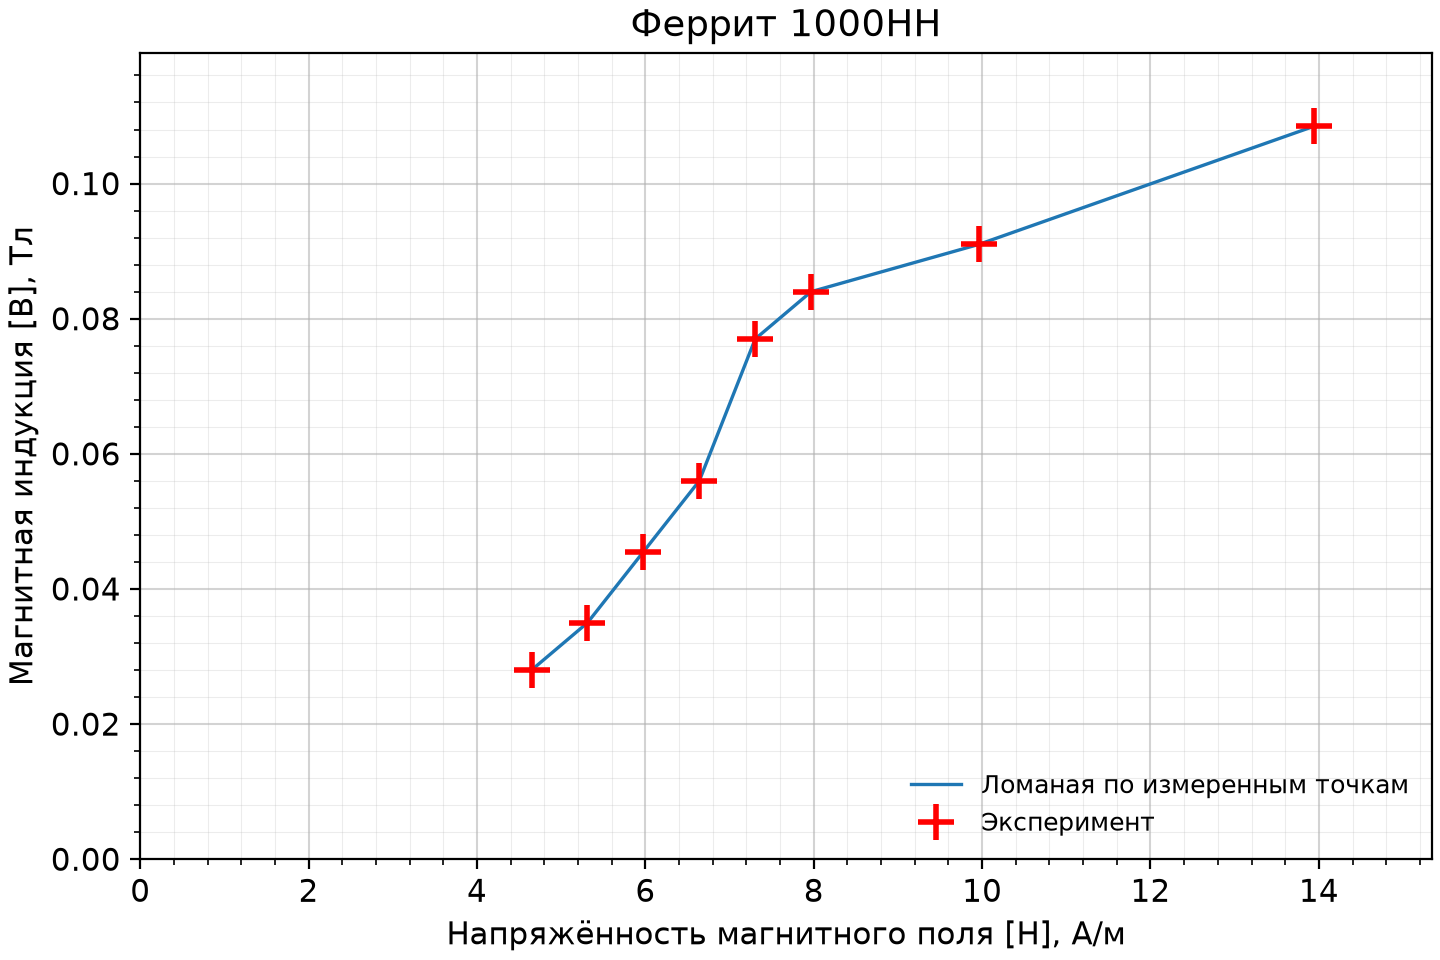
\includegraphics[width=0.85\textwidth]{images/B_of_H_3.png}
  \caption{Начальная кривая намагничивания (экспериментальные точки и соединяющие отрезки) феррита 1000НН $B(H)$}
  \label{fig:BH_3}
\end{figure}

\clearpage

\subsection{Дифференциальная магнитная проницаемость}

Дифференциальная магнитная проницаемость равна наклону
начальной кривой намагничивания:
\begin{equation}
  \mu_{\text{диф}}=\frac{dB}{dH}.
  \label{eq:mu}
\end{equation}
В используемом определении $\mu_{\text{диф}}$ имеет размерность
$\text{Гн/м}$ (то же, что $\text{Тл}\cdot\text{м/А}$).

Для оценки наклона построенных в п.~5.3 кривых вычислялись
угловые коэффициенты отрезков между соседними
экспериментальными точками:
\begin{equation}
  \mu_i^{\text{(отр)}}=
  \frac{B_{i+1}-B_i}{H_{i+1}-H_i}
  =\frac{\alpha_B}{\alpha_H}
   \frac{Y_{i+1}-Y_i}{X_{i+1}-X_i},
  \qquad H_{i+1}\ne H_i.
  \label{eq:mu_secant}
\end{equation}
Максимальную проницаемость оценивали по наибольшему конечному
наклону (\ref{eq:mu_secant}). Пары с одинаковыми $H$
исключались из этого расчёта.

Измерений вблизи $H=0$ нет, а состояние полного размагничивания
экспериментально не подтверждено. Поэтому начальную проницаемость
\emph{условно} оценивали по секущей от теоретического начала
координат до ближайшей измеренной точки $(H_{\min},B_{\min})$:
\begin{equation}
  \mu_{\text{нач}}^{\text{(оц)}}=
  \frac{B_{\min}}{H_{\min}}.
  \label{eq:mu_initial}
\end{equation}
Это условная оценка среднего наклона на участке от нуля до
$H_{\min}$, а не непосредственно измеренная производная
в точке $H=0$.

Например, для кремнистого железа Fe--Si первая по возрастанию поля
экспериментальная точка имеет $X=0{,}7$ дел. и $Y=1{,}0$ дел.
Используя коэффициенты $\alpha_H$ и $\alpha_B$,
получаем:
\begin{align*}
  \mu_{\text{нач},1}^{\text{(оц)}}
  &=\frac{\alpha_{B,1}\cdot1{,}0}{\alpha_{H,1}\cdot0{,}7}
    =7{,}2\cdot10^{-3}\ \text{Гн/м},\\
  \mu_{\max,1}^{\text{(оц)}}
  &=\frac{\alpha_{B,1}}{\alpha_{H,1}}
    \frac{1{,}2-1{,}0}{0{,}8-0{,}7}
    =1\cdot10^{-2}\ \text{Гн/м}.
\end{align*}

Аналогично найдены оценки для остальных образцов.
\begin{table}[H]
  \centering
  \caption{Оценки начальной и максимальной дифференциальной магнитной проницаемости}
  \label{tab:mu_results}
  \small
  \setlength{\tabcolsep}{5pt}
  \begin{tabular}{l c c c}
    \toprule
    Материал & \shortstack{$\mu_{\text{нач}}^{\text{(оц)}}$\\мГн/м} &
    \shortstack{$\mu_{\max}^{\text{(оц)}}$\\мГн/м} &
    \shortstack{Участок\\максимума} \\
    \midrule
    Кремнистое железо & 7,2 & 10 & 7--8 \\
    Пермаллой & 11 & 200 & 7--8 \\
    Феррит & 6,0 & 30 & 4--5 \\
    \bottomrule
  \end{tabular}
\end{table}

\clearpage

\subsection{Оценка погрешностей}

Погрешности рассчитывались методом распространения независимых
погрешностей:
\begin{equation}
 \Delta F=\sqrt{\sum_i\left(
   \frac{\partial F}{\partial x_i}\Delta x_i\right)^2}.
 \label{eq:error_propagation}
\end{equation}
Для характеристик петли $F=\alpha D/2$:
\begin{equation}
 \Delta F=|F|\sqrt{\delta_{\alpha}^2+
                 \left(\frac{\Delta D}{D}\right)^2},
 \qquad \delta_{\alpha}=\frac{\Delta\alpha}{|\alpha|}.
 \label{eq:error_loop}
\end{equation}

\begin{table}[H]
 \centering
 \caption{Магнитные характеристики с оценками погрешностей}
 \label{tab:results_errors}
 \small
 \setlength{\tabcolsep}{4.2pt}
 \begin{tabular}{c c c c c}
 \toprule
 Материал & $H_{\max}$, А/м & $B_s$, Тл & $H_c$, А/м & $B_r$, Тл \\
 \midrule
 Fe--Si & $201\pm5$    & $1{,}01\pm0{,}07$ & $61\pm4$     & $0{,}61\pm0{,}05$ \\
 НП50 & $20{,}6\pm0{,}4$ & $0{,}77\pm0{,}05$ & $17{,}0\pm0{,}4$ & $0{,}75\pm0{,}05$ \\
 1000НН & $12{,}0\pm0{,}4$ & $0{,}101\pm0{,}007$ & $6{,}6\pm0{,}3$ & $0{,}066\pm0{,}005$ \\
 \bottomrule
 \end{tabular}
\end{table}

Для постоянной времени получено
$\tau_{\text{эксп}}=(0{,}41\pm0{,}03)$~с.
Оценки начальной дифференциальной проницаемости:
\[
\begin{aligned}
 \mu_{\text{нач}}^{\text{Fe--Si}}&=(7{,}2\pm1{,}3)\cdot10^{-3}\ \text{Гн/м},\\
 \mu_{\text{нач}}^{\text{НП50}}&=(11{,}1\pm2{,}1)\cdot10^{-3}\ \text{Гн/м},\\
 \mu_{\text{нач}}^{\text{1000НН}}&=(6{,}0\pm1{,}2)\cdot10^{-3}\ \text{Гн/м}.
\end{aligned}
\]

\clearpage
\subsection{Сравнение с табличными данными}

Для сопоставления результатов использована табл.~13 приложения~В
лабораторного практикума МФТИ (с.~370)~\cite{ref:practicum}.
В ней приведены свойства магнитомягких ферромагнитных материалов:

\begin{table}[H]
 \centering
 \caption{Справочные характеристики магнитомягких материалов
 (таблица 13 практикума)}
 \label{tab:ref_compare}
 \small
 \setlength{\tabcolsep}{4.8pt}
 \begin{tabular}{l c c c c}
 \toprule
 Материал & $\mu_{\text{нач}}$ & $\mu_{\max}$ & $H_c$, А/м & $B_s$, Тл \\
 \midrule
 Fe--Si (4\,\% Si) & 500 & $7\,000$ & 40 & 1,95 \\
 Fe--Si (3\,\% Si) & $9\,000$ & $40\,000$ & 12 & 2,01 \\
 Пермаллой 45 & $1\,200$ & $3\,500$ & 5,6 & 1,60 \\
 Пермаллой 78 & $4\,000$ & $100\,000$ & 4 & 1,05 \\
 Феррит Ni--Zn & $10$--$2\,000$ & --- & $16$--$1\,600$ & $0{,}1$--$0{,}4$ \\
 Феррит Mn--Zn & $500$--$20\,000$ & --- & $4$--$100$ & $0{,}3$--$0{,}4$ \\
 \bottomrule
 \end{tabular}
\end{table}

Для исследованного Fe--Si концентрация кремния не указана,
поэтому приведены оба состава из справочной таблицы.
Марки пермаллоя НП50 и феррита 1000НН в ней отсутствуют:
для них представлены справочные данные других пермаллоев
и двух классов ферритов. Точное совпадение характеристик
этих материалов не предполагается.

Экспериментальное коэрцитивное поле Fe--Si
$(61\pm4)$~А/м превышает значения $12$ и $40$~А/м,
а индукция насыщения $(1{,}01\pm0{,}07)$~Тл меньше
значений $1{,}95$ и $2{,}01$~Тл.
Для пермаллоя НП50 получено $H_c=(17{,}0\pm0{,}4)$~А/м
и $B_s=(0{,}77\pm0{,}05)$~Тл; в таблице для
пермаллоев 45 и 78 даны $H_c=5{,}6$ и $4$~А/м,
$B_s=1{,}60$ и $1{,}05$~Тл соответственно.
Для феррита 1000НН получено $H_c=(6{,}6\pm0{,}3)$~А/м
и $B_s=(0{,}101\pm0{,}007)$~Тл;
справочные диапазоны зависят от типа феррита.

Значения $\mu_{\text{нач}}$ и $\mu_{\max}$ в практикуме
являются \emph{относительными безразмерными} проницаемостями:
$\mu_{\text{отн}}=\mu_{\text{диф}}/\mu_0$.
Для наших оценок начального наклона получаем:
\[
\begin{aligned}
 \mu_{\text{отн,нач}}^{\text{Fe--Si}} &= (5{,}7\pm1{,}0)\cdot10^3,\\
 \mu_{\text{отн,нач}}^{\text{НП50}} &= (8{,}8\pm1{,}7)\cdot10^3,\\
 \mu_{\text{отн,нач}}^{\text{1000НН}} &= (4{,}8\pm1{,}0)\cdot10^3.
\end{aligned}
\]

Прямое сопоставление ограничено: экспериментальные оценки
проницаемости найдены по секущим, а табличные значения
относятся к производной в начале кривой намагничивания.
Кроме того, измерения проводились при переменном поле
частотой 50~Гц и не обязательно соответствуют условиям,
при которых получены справочные характеристики.

\clearpage
\section*{Вывод}

В работе исследованы три материала: кремнистое железо Fe--Si,
пермаллой Fe--Ni НП50 и феррит 1000НН.

Рассчитана максимальная напряжённость магнитного поля:
\[
\begin{aligned}
 H_{\max}^{\text{Fe--Si}} &=(201\pm5)\ \text{А/м},\\
 H_{\max}^{\text{НП50}} &=(20{,}6\pm0{,}4)\ \text{А/м},\\
 H_{\max}^{\text{1000НН}} &=(12{,}0\pm0{,}4)\ \text{А/м}.
\end{aligned}
\]

Рассчитана индукция насыщения:
\[
\begin{aligned}
 B_s^{\text{Fe--Si}} &=(1{,}01\pm0{,}07)\ \text{Тл},\\
 B_s^{\text{НП50}} &=(0{,}77\pm0{,}05)\ \text{Тл},\\
 B_s^{\text{1000НН}} &=(0{,}101\pm0{,}007)\ \text{Тл}.
\end{aligned}
\]

Рассчитано коэрцитивное поле:
\[
\begin{aligned}
 H_c^{\text{Fe--Si}} &=(61\pm4)\ \text{А/м},\\
 H_c^{\text{НП50}} &=(17{,}0\pm0{,}4)\ \text{А/м},\\
 H_c^{\text{1000НН}} &=(6{,}6\pm0{,}3)\ \text{А/м}.
\end{aligned}
\]

Рассчитана остаточная магнитная индукция:
\[
\begin{aligned}
 B_r^{\text{Fe--Si}} &=(0{,}61\pm0{,}05)\ \text{Тл},\\
 B_r^{\text{НП50}} &=(0{,}75\pm0{,}05)\ \text{Тл},\\
 B_r^{\text{1000НН}} &=(0{,}066\pm0{,}005)\ \text{Тл}.
\end{aligned}
\]

Оценена начальная дифференциальная магнитная проницаемость:
\[
\begin{aligned}
 \mu_{\text{нач}}^{\text{Fe--Si}} &=(7{,}2\pm1{,}3)\cdot10^{-3}\ \text{Гн/м},\\
 \mu_{\text{нач}}^{\text{НП50}} &=(11{,}1\pm2{,}1)\cdot10^{-3}\ \text{Гн/м},\\
 \mu_{\text{нач}}^{\text{1000НН}} &=(6{,}0\pm1{,}2)\cdot10^{-3}\ \text{Гн/м}.
\end{aligned}
\]

Экспериментально определена постоянная времени интегрирующей цепочки:
\[
 \tau_{\text{эксп}}=(0{,}41\pm0{,}03)\ \text{с}.
\]



\begin{thebibliography}{9}
\bibitem{ref:practicum}
Лабораторный практикум по общей физике.
Т.~2. Электричество и магнетизм / под ред.
А.~В.~Максимычева и М.~Г.~Никулина. ---
2-е изд. --- М.: МФТИ, 2019. ---
Приложение~В, табл.~13, с.~370.
\end{thebibliography}

\end{document}
